% !TeX document-id = {1d88a3b2-9b5b-461b-9b0a-590d1c20474b}
% !TeX TXS-program:compile = txs:///pdflatex/[--shell-escape]
\documentclass[border={0 -1mm 0 -1mm}]{standalone}
\usepackage{amsmath,amsfonts,amssymb}
\usepackage{tikz,pgfplots}
\usetikzlibrary{arrows,arrows.meta,bending,calc,decorations,shadings,shadows,shapes,shapes.arrows,shapes.geometric}
\usetikzlibrary{calc,fadings,decorations.pathreplacing}
\usepgfplotslibrary{units,fillbetween,groupplots,colorbrewer}
\usetikzlibrary{pgfplots.colorbrewer,}
\usepackage{pgfplotstable}

\pgfdeclareplotmark{*)}
{\shade[draw=red!60!black,ball color=red!70,opacity=0.5] (0,0) circle [radius=2pt];}


\newcommand*{\xMin}{0}%
\newcommand*{\xMax}{10}%
\newcommand*{\yMin}{0}%
\newcommand*{\yMax}{7}%

\begin{document}
	
	\begin{tikzpicture}
%		
%				\draw[step=.5cm,gray,very thin,opacity=0.1] (0,0) grid (\xMax,\yMax);
%				 \foreach \i in {\xMin,...,\xMax} {
%					\draw [very thin,gray] (\i,\yMin) -- (\i,\yMax)  node [below] at (\i,\yMin) {$\i$};
%				}
%				\foreach \i in {\yMin,...,\yMax} {
%					\draw [very thin,gray] (\xMin,\i) -- (\xMax,\i) node [left] at (\xMin,\i) {$\i$};
%				}
			
		
		 
		 

		 
		 \node[anchor=west,blue](fs) at (8,1.25) {First sublattice};
		 
		 \node[anchor=west,blue](ss) at (8,2.7) {Second sublattice};
		 
		 \draw[-{Stealth[scale=1]}, line width=0.5mm] (6.1,0.7) to [out=0,in=180](fs);
		 \draw[-{Stealth[scale=1]}, line width=0.5mm] (5.7,1.6) to [out=0,in=180](ss);
	

	 \node[anchor=center,opacity=1] at (3.5,3.5) {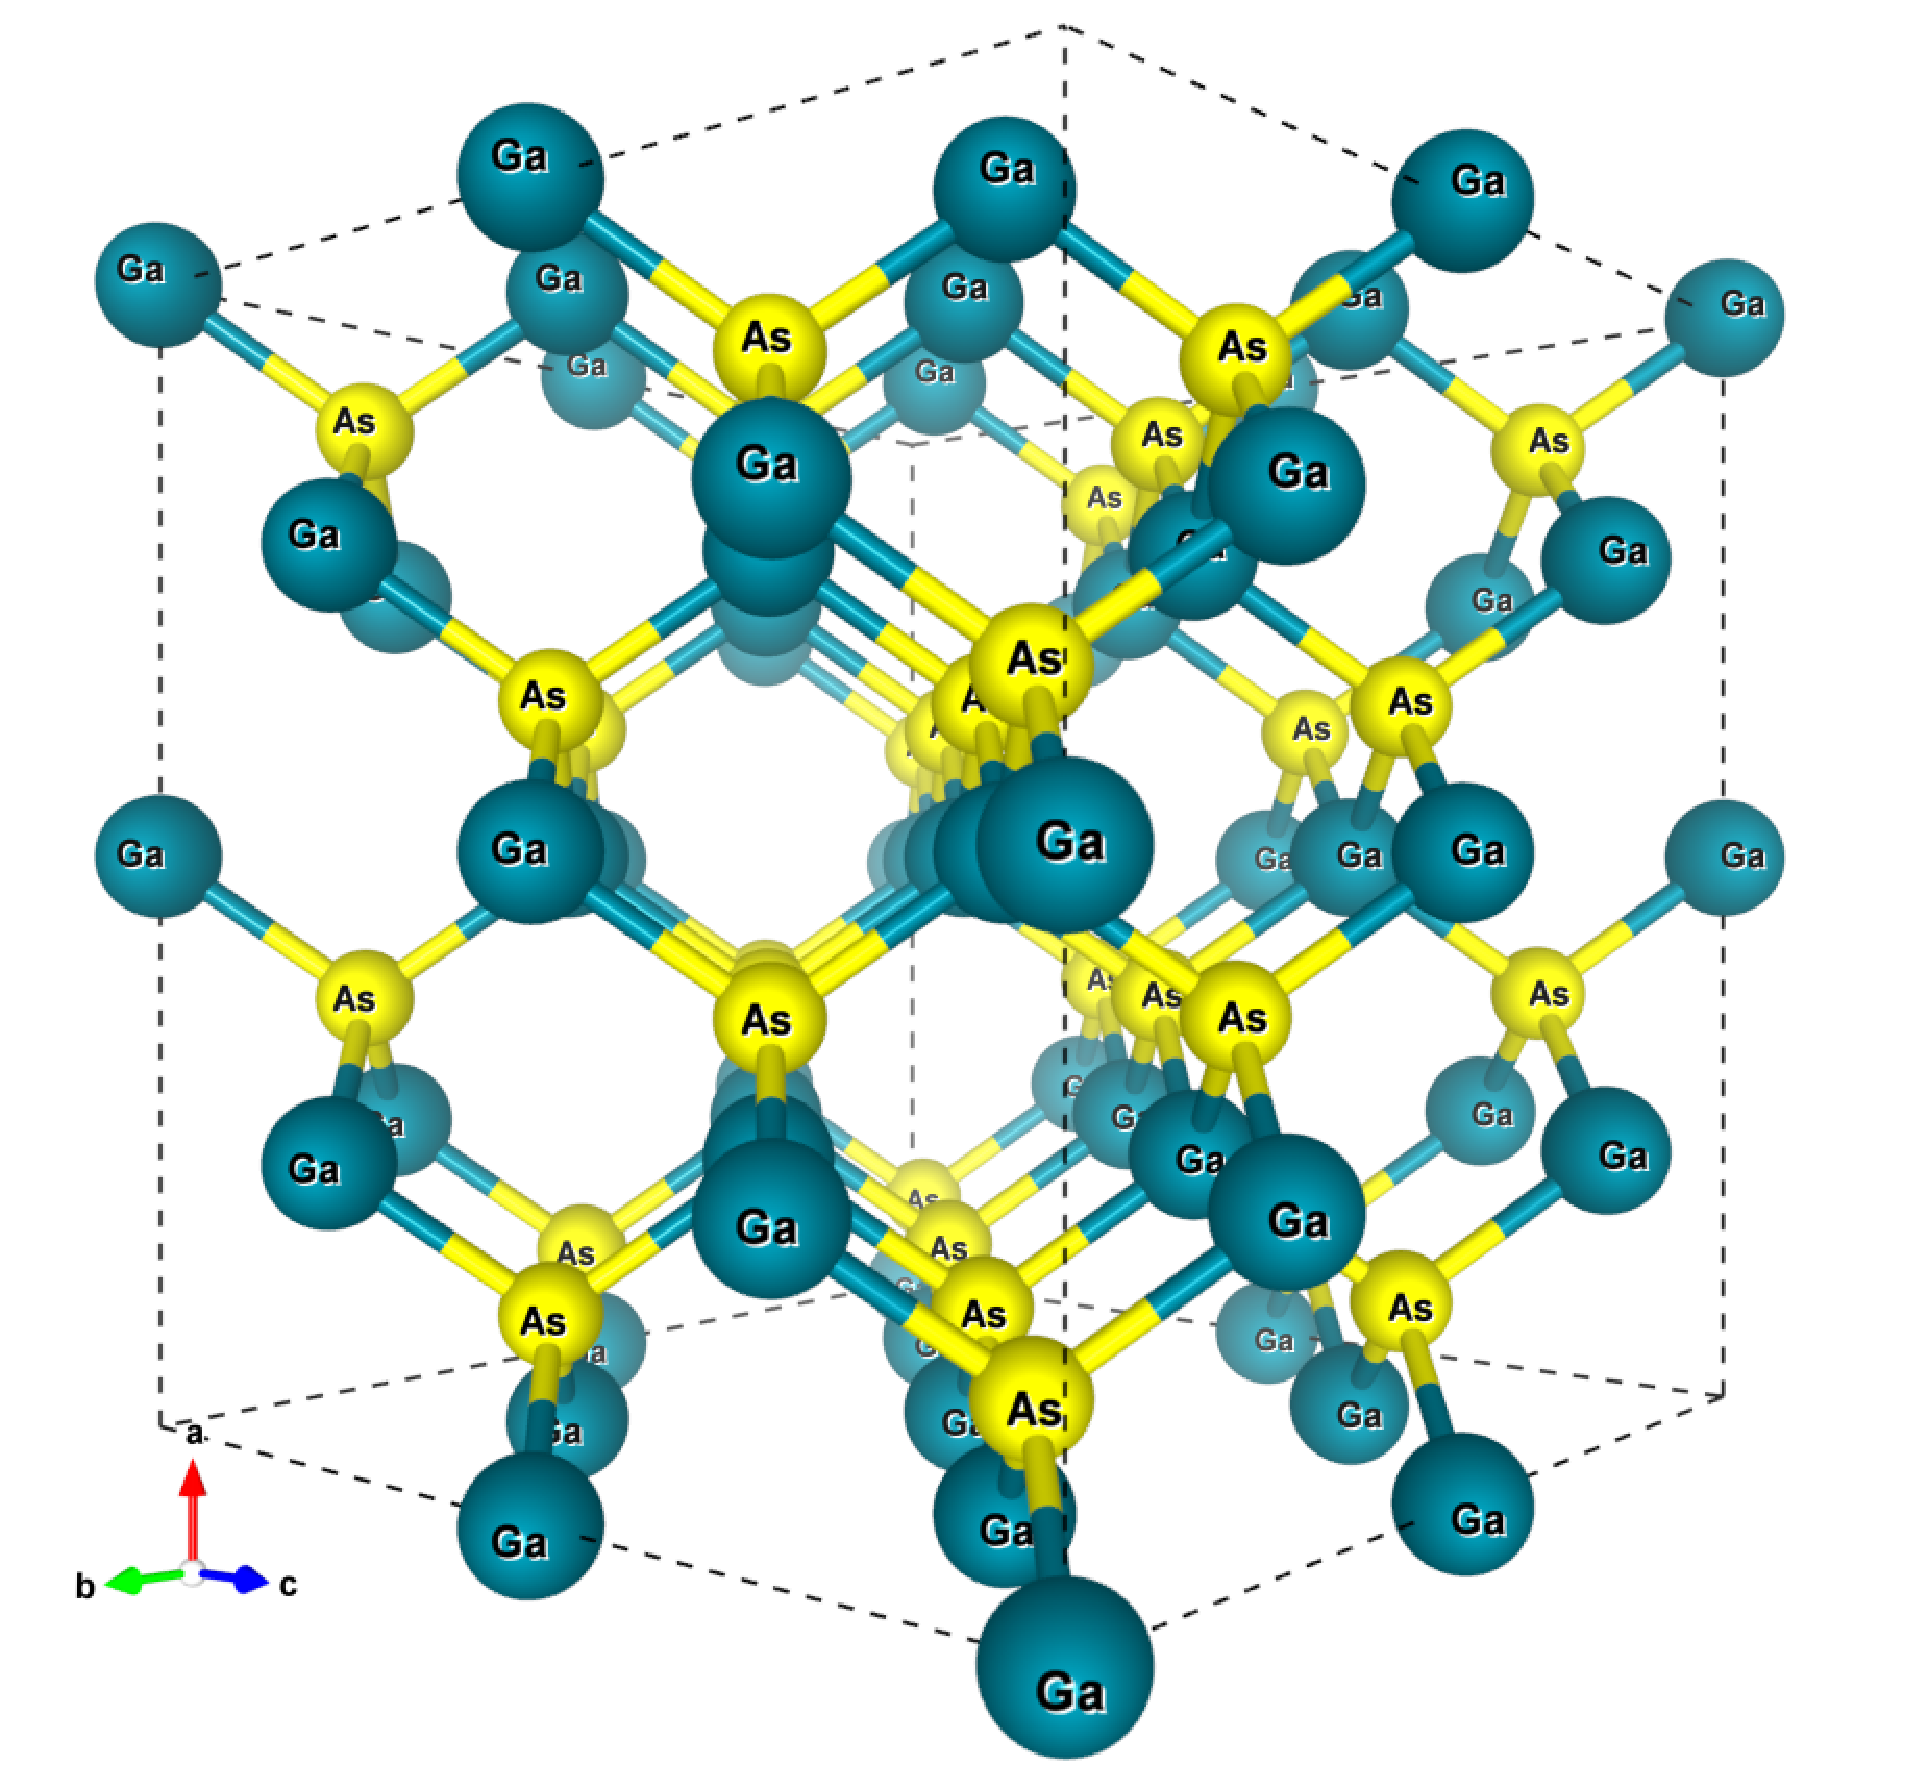
\includegraphics[width=0.7\linewidth]{/media/labfiles/ruco/phd-ssp/phd-codes/atom-structures/gaas-bulk-01.pdf}};
	\end{tikzpicture}
	
	
	
\end{document}